\section{Preliminaries}
\label{sec:related}

In this section, we first summarize and review some related preliminary works of on-chip power grid EM-induced IR drop analysis and mitigation approaches.

\subsection{Full-chip EM-induced IR drop analysis}
\label{subsec:emspice}
As mentioned in the previous section, EM is a physical phenomenon that can lead to resistance increase or even open-wire segments.  The IR drop of the power grid wires may change due to the EM-induced aging effect. This means we have to consider the power girds IR drop as time-varying characters ~\cite{SunYu:TDMR'20, Huang:TCAD'15, Chatterjee:2018TCAD,SukharevNajm:2018TDMR}. 
On the other hand, the failed wire segments change the current distributions of all the interconnect wires, which may further accelerate the failure process. Hence, to emulate the on-chip power grid IR-drop after aging effect, one has to consider the interplay between the two physics: electrical characteristics and hydrostatic stress in the interconnect wires.

{\it EMspice}~\cite{SunYu:TDMR'20,EMspiceSourceCode} is an open source tool that conducts the full-chip power grid network coupled EM-IR drop simulation with the dynamic interplay between the hydrostatic stress and electronic current/voltage. It solves the coupled time-varying partial differential equations in the time domain to obtain the stress evolution, and finally reports resulted IR drop and EM failure hotspots at the target aging time, such as 10 years.  The tool consists of a finite difference time domain (FDTD) solver for EM stress and a linear network DC solver for IR drop. The linear network IR drop solver passes time-dependent current densities and P/G layout information to the finite difference time domain (FDTD) EM solver, and the FDTD EM solver provides the IR drop solver with new resistance information. These two simulations are coupled together and must be solved together, which can be described as

%\begin{align}
%	\label{eq:em}
%		&{\bf C} \dot{\sigma}(t)  = {\bf A} \sigma(t) + {\bf P}I(t),  \\
%		&\mathcal{V}_v(t)  = \int_{\Omega_L}\frac{\sigma(t)}{B}d\mathcal{V},  \\ 
%		&{\bf M}(t) \times u(t)  = {\bf P} I(t), \\
%		&{\bf \sigma}(0)  = [\sigma_1(0), \sigma_2(0), ..., \sigma_n(0)] \,\, ,at \,\, t = 0 
%\end{align}

\begin{align}
	\label{eq:em}
	\begin{split}
		&{\bf C} \dot{\sigma}(t)  = {\bf A} \sigma(t) + {\bf P}I(t),  \\
		&\mathcal{V}_v(t)  = \int_{\Omega_L}\frac{\sigma(t)}{B}d\mathcal{V},  \\ 
		&{\bf M}(t) \times u(t)  = {\bf P} I(t), \\
		&{\bf \sigma}(0)  = [\sigma_1(0), \sigma_2(0), ..., \sigma_n(0)] \,\, ,at \,\, t = 0 
	\end{split}
\end{align}
In the above equations, ${\bf M}(t)$ is the time varying power grid conductance matrix, as the resistance changes due to the EM failure process. ${{\bf P}}$ is the input matrix and I(t) represents the current sources from the chip. ${{\bf C}}$ is the identity matrix and ${{\bf A}}$ is a coefficient matrix. $\sigma_{n}(0)$ denotes the initial stress at time step $t = 0$, for node $n$. For each new time step, the stress from previous simulation step is used as the initial condition. Such iterative coupled analysis on long target lifetime can be extremely time consuming for very large power grid networks.

There are some research efforts to facilitate the IR drop/EM-aware IR drop analysis by leveraging machine learning based approaches to build the surrogate models, including ~\cite{LinFang:2018vts,Fang:2018dynireco,HoKahng:ICCAD'19,Xie:2020powernet,Sachin:ASPDAC'21} to reduce the evaluation time during the physical design process.  Lin {\it et al.}~\cite{LinFang:2018vts} tried to extract power and physical features from cells and layouts to conduct the full-chip dynamic IR drop analysis. Fang {\it et al.}~\cite{Fang:2018dynireco} proposed to training the models for the localized layout region to improve the scalability.  A convolutional neural network (CNN) model which features incorporating design-dependent features during pre-processing was proposed by Xie {\it et al.}~\cite{Xie:2020powernet}. Ho {\it et al.}~\cite{HoKahng:ICCAD'19} proposed incremental IR drop prediction and mitigation by applying more electrical and physical features for the gradient boosting framework training. Chhabria {\it et al.}~\cite{Sachin:ASPDAC'21} proposed {\it IREDGe}, which is a CNN-based generative network method to predict on-chip IR drop contours with image-to-image and sequence-to-sequence translation tasks.
%These machine learning methods indeed have achieved significant progress in IR drop estimation, but either none of them takes EM aging effects into consideration
 %Recently Zhou {\it et al.}~\cite{ZhouJin:ICCAD'20} proposed an EM-aware IR drop analysis framework based on conditional GAN model.
Recently Zhou {\it et al.} \cite{ZhouJin:ICCAD'20} considered more accurate physics-based EM effects into IR drop to build such surrogate models. It adopted the GAN-based structure to model the resulting EM-aware IR drops.  This method regards the time, 2D power grid structure with input current and voltages as input images (series of images) and outputs the voltage map images. Such surrogate model can help to speedup wire sizing by fast EM-aware IR drop estimation and the sensitivity of objective functions with respect to the wire geometries. It was initially applied to localized PDN optimization then has been extended to full-chip optimization~\cite{HanLiu:TCAD'22-23}.
 %However GAN-based strategies have some drawbacks, such as training collapse due to the need to optimize the opposing objectives of the generator and discriminator. 
% ~\cite{ZhouJin:ICCAD'20} also demonstrates the trained ML models can help accelerating the PDN optimization task by providing the sensitivity of objective EM-induced IR-drop with respect to the initial wire resistances. It was initially applied to localized PDN optimization then has been extended to full-chip optimization~\cite{HanLiu:TCAD'22-23}.
However the GAN-based models suffers from the difficulties to train both the generator and discriminator together. Also the deterministic latent variable encoding and decoding approach used by GAN model, makes the latent space lack of continuity and interpretability, less generative capability (due to non-regulated latent space), eventually effect the prediction accuracy.


\subsection{Existing EM-aware PDN optimization}
 \label{subsec:exist_pgfix}
 % There have been a number of works proposed recently on wire segment sizing of power grid networks in order to fix the EM failures and IR drop considering the multi-segment interconnect wires. Zhou {\it et al.}~\cite{ZhouSun:ASPDAC'18,ZhouSun:TVLSI'19} proposed a power grid network sizing method based on the multi-segment EM immortality check criteria. It automatically considers all the wire segments and their interactions in an interconnect tree. However, the EM immortality constrained optimization is still conservative as it requires all the interconnect trees to be immortal, i.e., void nucleations are not allowed. Chang {\it et al.}~\cite{ChangBaranwal:ASPDAC'18} proposed a learning-based EM violation waiver system, which investigates every EM violation and takes an expert decision to either ignore the violation (waive-off) or resolve it (must-fix) in the design. However, this system cannot take the violation fix action.
 Besides the full-chip aging-aware IR-drop estimation, one also need to fix or alleviate the excessive IR-drop to ensure a robust PDN design. Many past research apply nonlinear methods~\cite{ChBr:TCAD'88,DuMa:DAC'89,Tan:DAC'99,Wang:TCAD'05,ZhouSun:TVLSI'19, Sukharev:2019pg} to properly size the PDN wires. The goal of these optimization strategies is to meet the IR drop requirement at the target lifetime or extend the main time to failure (MTTF) with minimize metal routing area.

The SLP-based method was proposed first in~\cite{Tan:DAC'99} based on Black's equation. Then this method was extended to consider multi-segment wires ~\cite{ZhouSun:ASPDAC'18}. But this method can be too conservative as it requires all the wires to be immortal after optimization. Although this method has been extended to consider a targeted lifetime by allowing some wires to fail and optimizing the rest of the wires~\cite{ZhouSun:TVLSI'19}.  Recently \cite{Sukharev:2019pg} proposed to directly optimize EM-induced IR drops on the time-varying power grid networks EM caused by EM-induced aging using SLP method. However, the EM-induced IR drop are still computed by solving Korhonen equations, and the sensitivities of the IR drop with respect to the wires are computed through matrix solving method.  
%Since it models the power grid network as a nonlinear time-varying system,  \cite{Sukharev:2019pg} need s to repeat at each time step. 
The solving process is severely time-consuming, especially when the power grid is large.

%To solve the optimization problem, we need two main inputs: v(T=t) and dv/ds.  There are some methods to compute dv/ds, such as adjoint network method. Vxx also proposed a matrix solving method, The main drawback is, the dv/ds has to be computed for each



 % This method aims to re-size the individual wires to meet the target IR drop criteria. The approach applies successive linear programming method, which iteratively expand a non-linear problem to a linear space and then optimize it. Each iteration contains the following steps: first linearize the nodes voltage drop around the current \textcolor{blue}{grid topology(wrong term)}, then determine the gradient descent direction at the current solution point through partial differential computation, finally find the updated solution point by solving a linear programming problem. Clearly this numerical computation method takes a huge amount of workload, hence the speed and scalability are the main issues.
 % We hereby propose our DNN-based machine learning method to accelerate this optimization approach. We replace the

\subsection{Variational Autoencoder}
\label{subsec:vae_intro}
In this paper, we adopt VAE~\cite{Diederik:arxiv'22} as the machine learning models for the EM-aware IR drop estimations. 
VAE follows the similar structure of autoencoder(AE).

The traditional AE structure, as shown in Fig.\ref{fig:ae}, includes encoder and decoder structures. A input will be encoded to low dimensional latent variables by the encoder, and then decoded to the output by the decoder.  
The GAN model adopts the standard AE as a \textit{generator} to generate the result, and use an additional binary output CNN as the discriminative network only in the training stage to better train the autoencoder. 


\begin{figure}[htp]
	\centering
	\subfigure[]{
		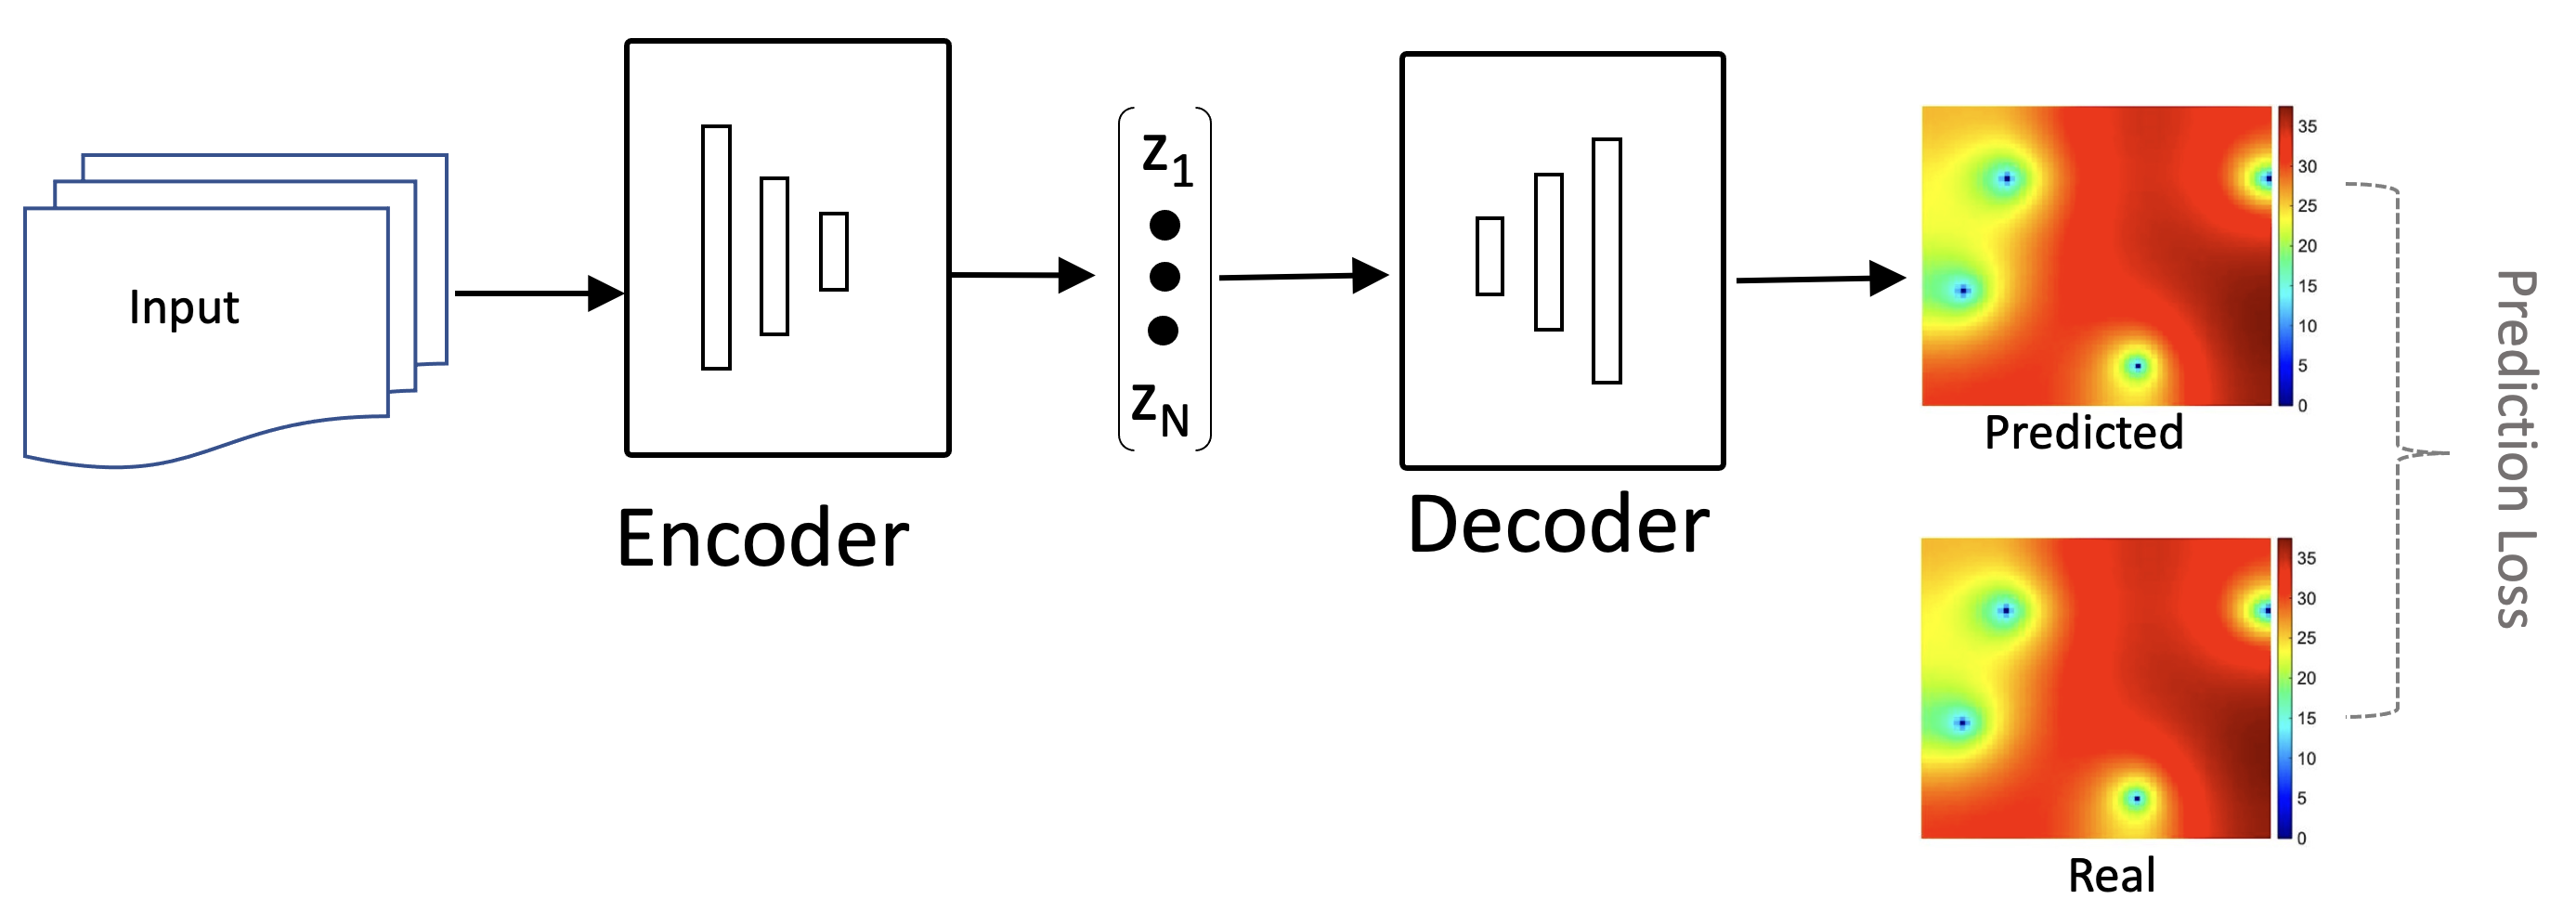
\includegraphics[width=0.9\columnwidth, height = 3cm]{./figs/ae_brief.eps}
		\label{fig:ae}}
	\subfigure[]{
		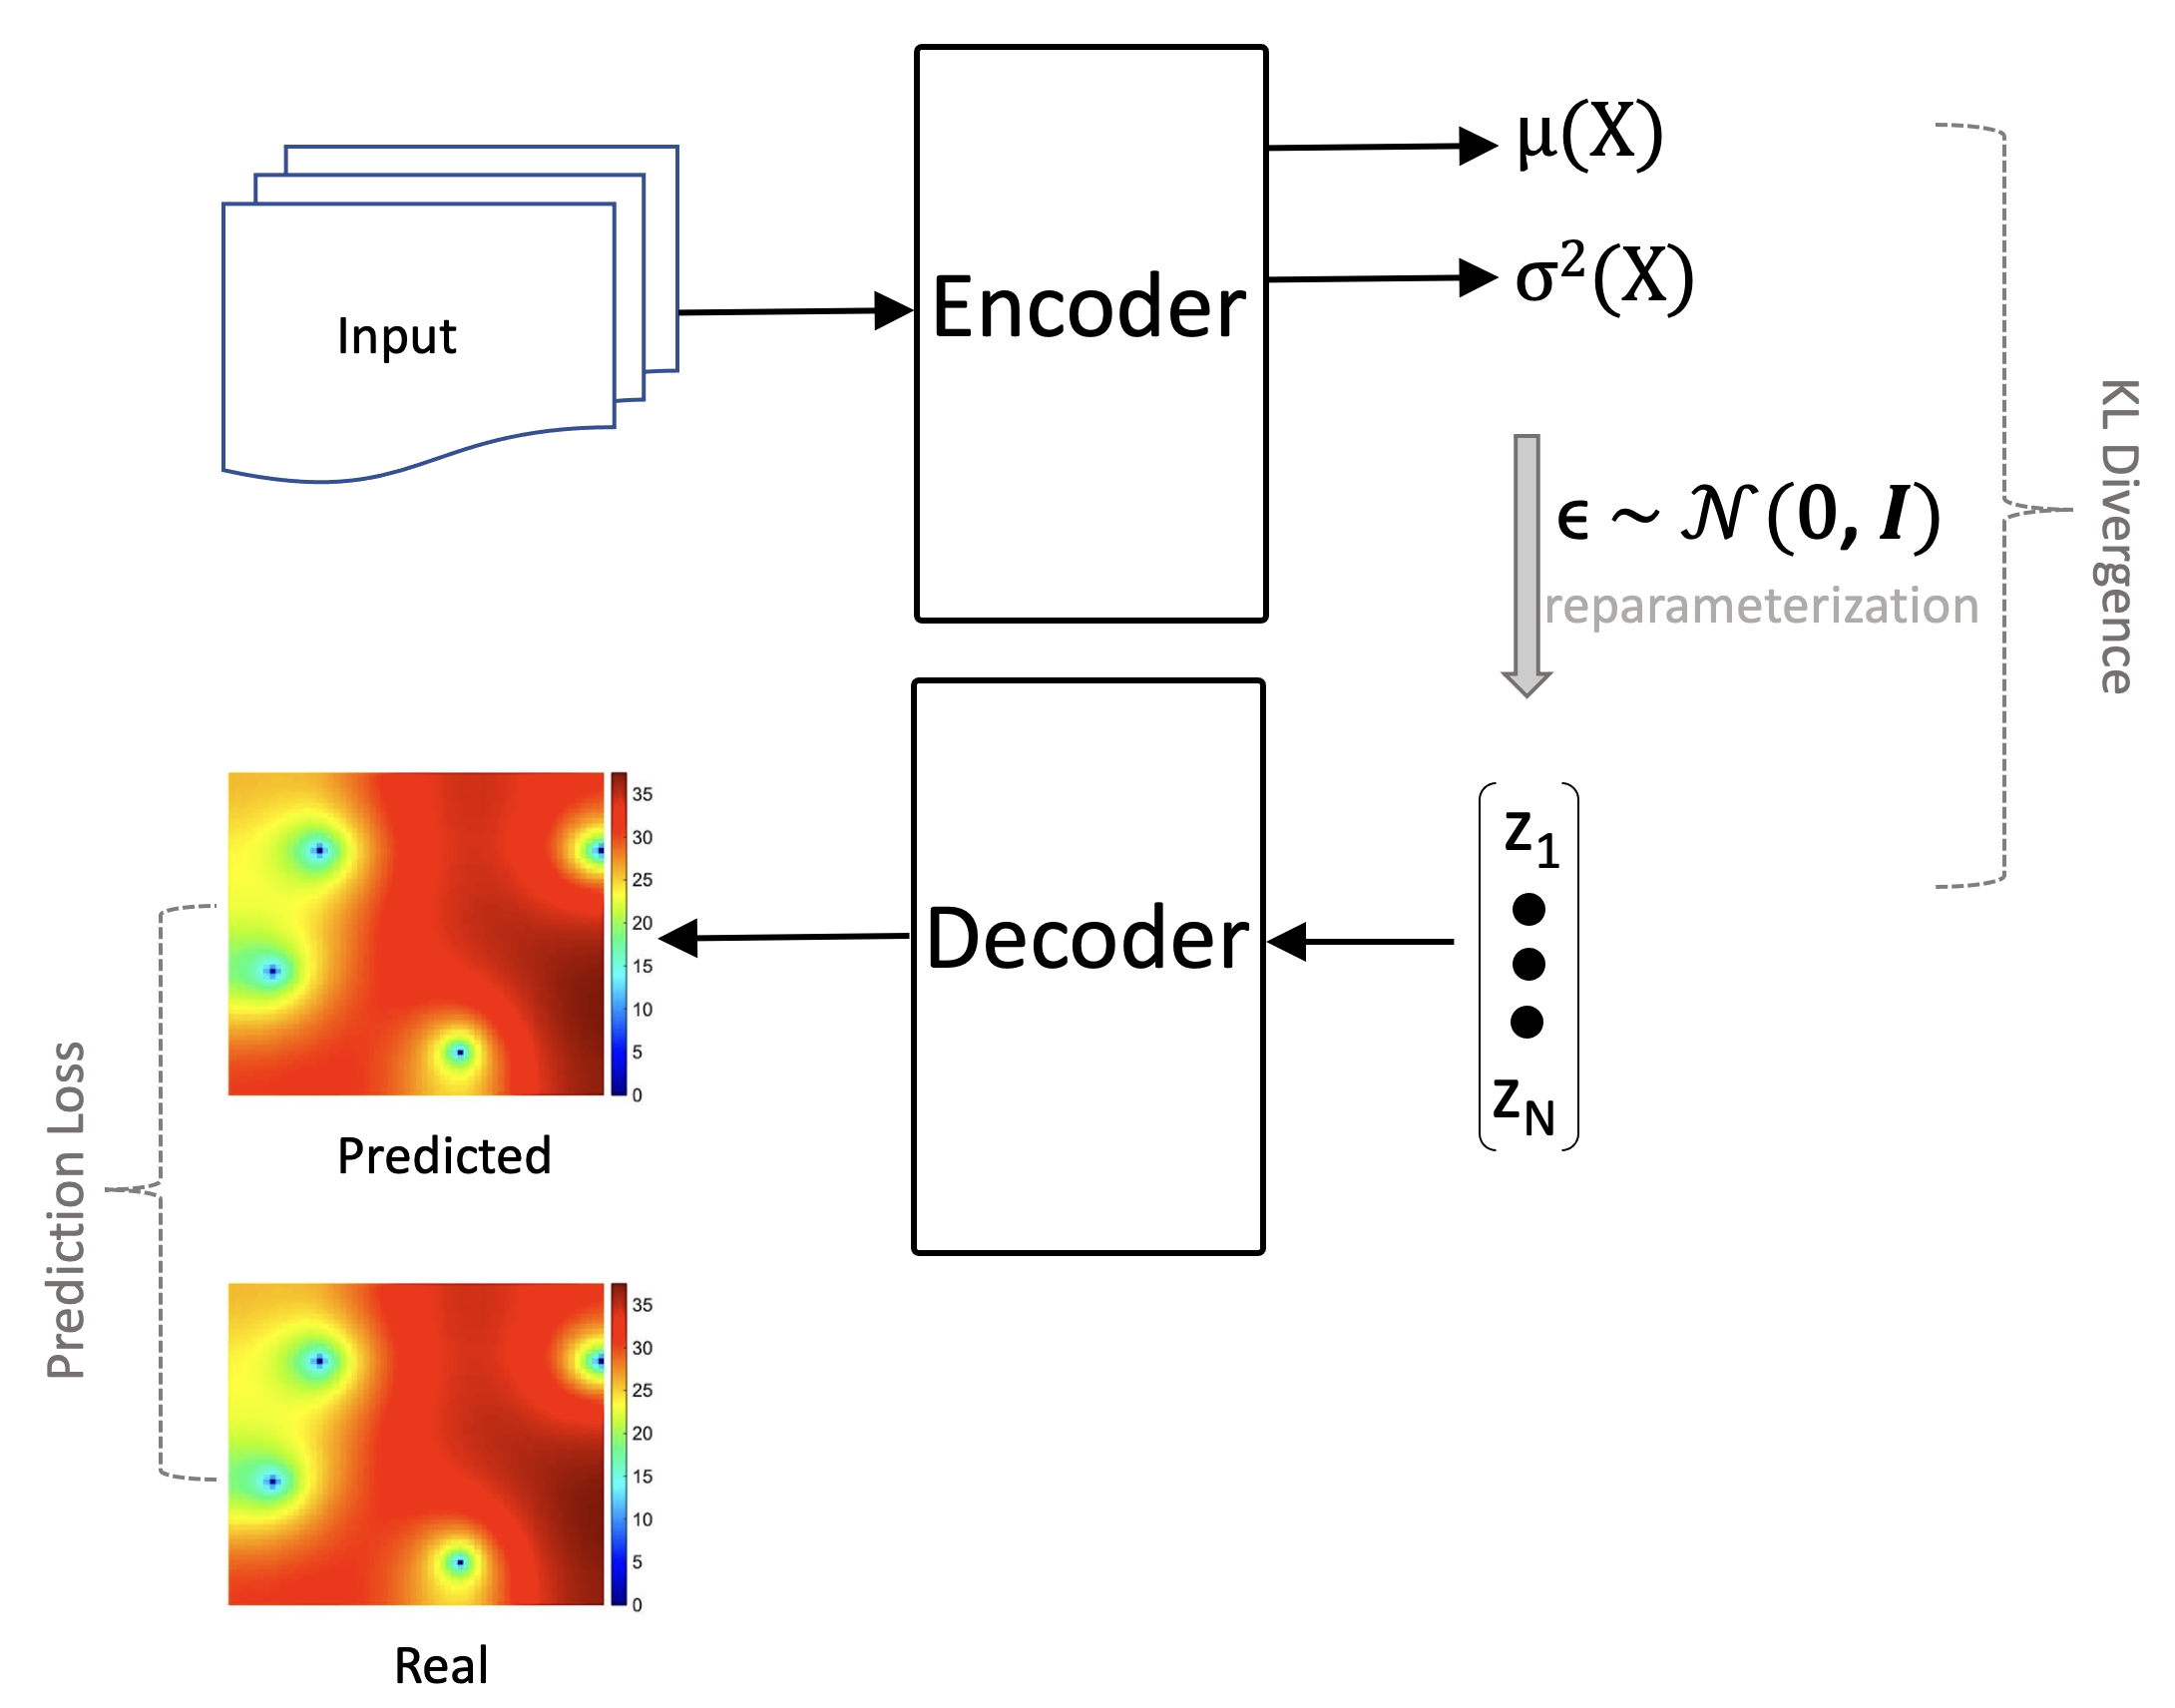
\includegraphics[width=0.8\columnwidth]{./figs/vae_brief.eps}
		\label{fig:vae}}
	\caption{(a) Architecture of an auto encoder (b)Architecture of a variational auto encoder }
	\label{fig:compare_ae_vae}
\end{figure}


 
Variational autoencoder, as shown in  Fig.\ref{fig:vae}, is a type of unique generative model derived from the standard autoencoder, which are used to generate new data that is similar to the input data they're trained on. 
Compared to traditional autoencoder structure, VAE does not directly encode the input to a determined latent variable, instead its encoded to a distribution over the latent space $Q(Z|X)$, and then sampling from this distribution to generate a latent variable for the decoder. This step is crucial to the VAE's some crucial characteristics over AE and AE-based GAN model, such as Interpretability of Latent Space, and Training Stability.
Interpretability of Latent Space means that the latent space is smooth and interpretable, enabling nice properties like the ability to interpolate between different points in the latent space and generate new samples that exhibit a smooth transition between the characteristics of the original points. On the other hand, AE does not explicitly enforce such a structure, making the latent space less interpretable and interpolations might not always produce meaningful outputs. 
Usually the VAE latent variable $z$ is generated using a reparameterization approach to ensure the model back propagation with gradient descent . We denote the mean of $Q(Z|X)$ as $\mu$ and the standard deviation as $\sigma$, and sample $\epsilon \sim \mathcal{N}(\textbf{0}, \textbf{I} ) $, then compute z as equation.\eqref{eq:z_compute}:

\begin{equation}
	\label{eq:z_compute}
	z = \mu(\textit{X}) + \sigma \ast \epsilon(\textit{X})
\end{equation}


The Loss function for a VAE contains two parts. The first part is the \textit{reconstruction loss}, also called \textit{prediction loss} when the input and output are expected to be different. The prediction loss measures the difference between the decoded result $\hat{y} = P(\hat{y}|z)$ and label $y$, encourages the decoded output data to be similar to the label. As our data is continuous, we allocate the mean squared error (MSE) for the prediction loss evaluation \eqref{eq:vae_MSE_loss}, where N is the total number of output pixels.
\begin{equation}
	\label{eq:vae_MSE_loss}
	\textit{MSE}(y, \hat{y}) = \frac{1}{N} \sum_{1}^{N} ( y - \hat{y})^{2}
\end{equation}
The second part is the \textit{Kullback-Leibler (KL) divergence} between the latent variable distribution $Q(z|x)$ output by the encoder and a chosen prior distribution, usually a standard multivariate gaussian distribution $\mathcal{N}(\textbf{0}, \textbf{I})$. The \textit{KL divergence} measures how one probability distribution is different from a second, which acts as a regularization term to force the encoded latent distribution from the given training dataset to be close to a standard normal distribution, and encourage the network to use the latent space efficiently. 
The \textit{KL divergence} in VAE can be written as:
%$\mathcal{N}(\mu_{x}, \sigma_{x}^{2})$ 

\begin{equation}
	\label{eq:vae_KLD_loss}
	D_{KL}( \mathcal{N}(\mu_{x}, \sigma_{x}^{2}) ~ || ~ \mathcal{N}(\textbf{0}, \textbf{I} ) )  = \dfrac{1}{2} (-\log\sigma^{2} + \mu^{2} + \sigma^{2} - 1)
\end{equation}

Hence the training target is to minimize the total loss:
\begin{equation}
	\label{eq:vae_total_loss}
	%\min_{\theta}  \{  \textit{MSE} (y , \hat{y} )   ~ + ~  D_{KL}( \mathcal{N}(\mu_{x}, \sigma_{x}^{2}) ~ || ~ \mathcal{N}(\textbf{0}, \textbf{I} ) )  \}
	\min  \{ \textit{MSE} (y, \hat{y})  ~ + ~  D_{KL}( \mathcal{N}(\mu_{x}, \sigma_{x}^{2}) ~ || ~ \mathcal{N}(\textbf{0}, \textbf{I} ) )  \}
\end{equation}



%\begin{figure}[htp]
%	\centering
%	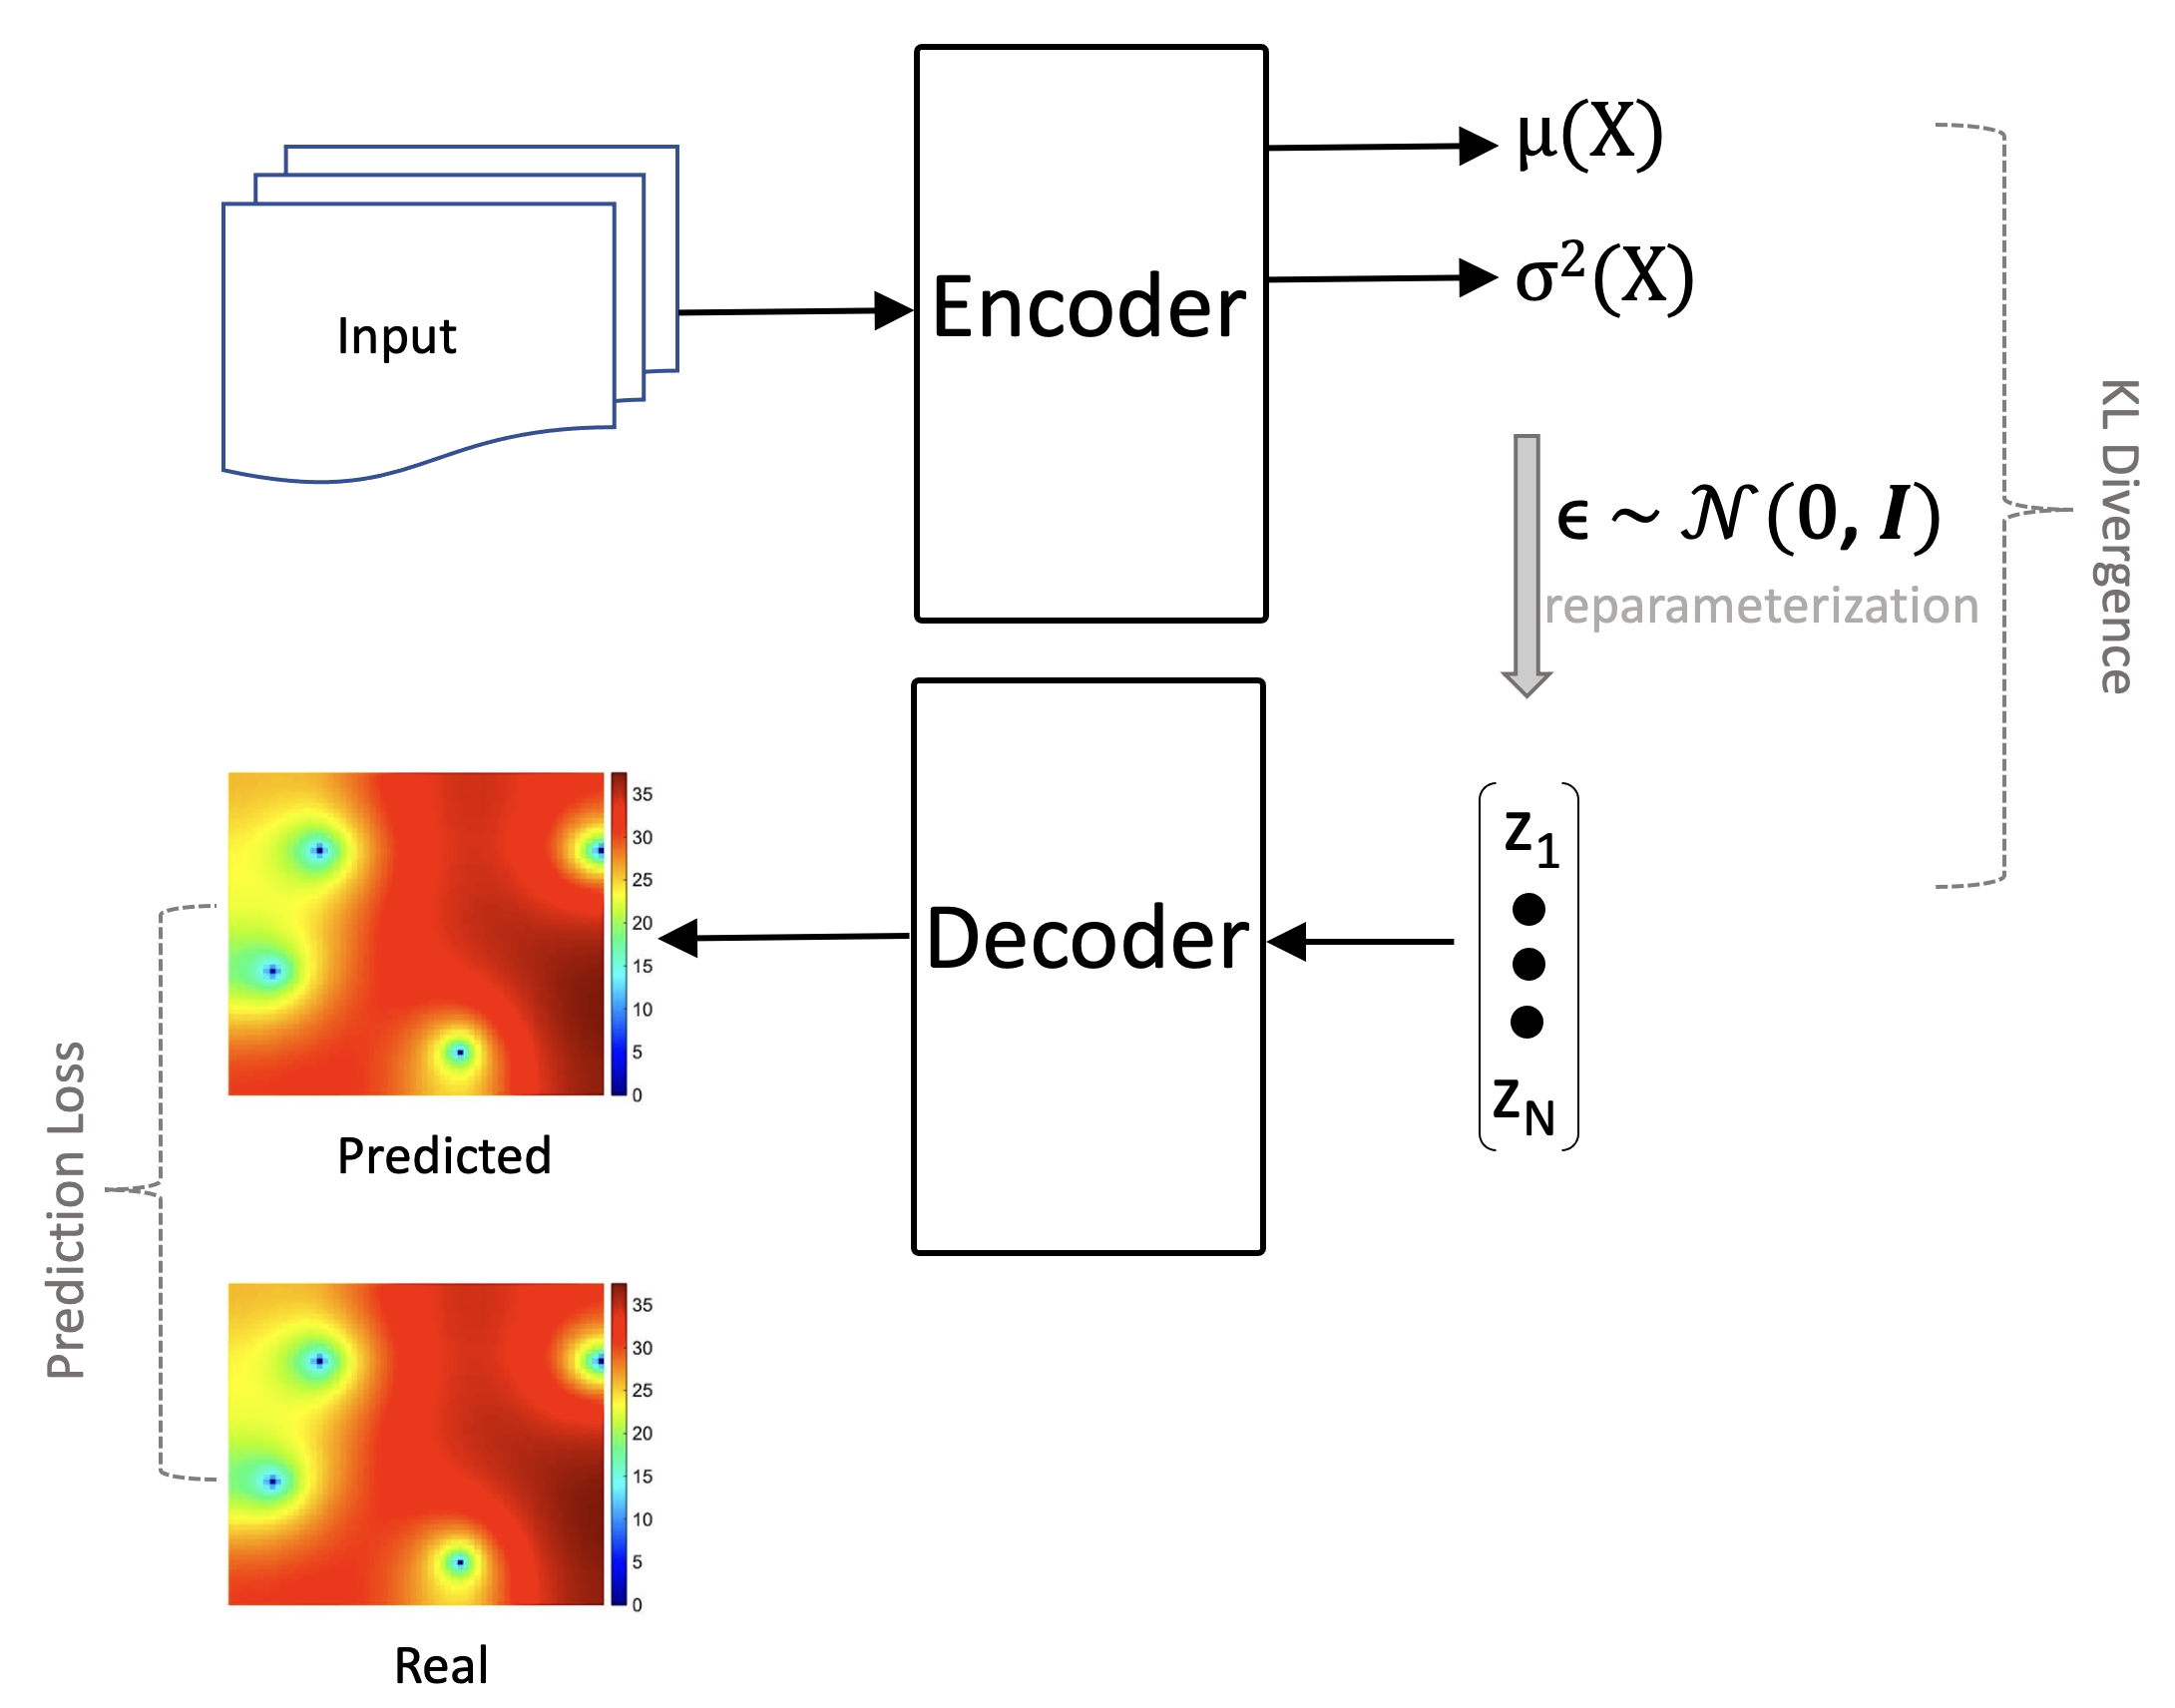
\includegraphics[width=0.8\columnwidth]{./figs/vae_brief.eps}
%	\label{fig:ae_vs_vae}
%	\caption{Architecture of a variational auto encoder }
%	\label{fig:vae}
%\end{figure}

